To create a realistic simulator, a physics-based simulator, Gazebo, was used. This simulator can simulate the dynamics of the system in real time, as well as the sensors employed, and it is easy to integrate with both ROS and ROS2. This integration was a key requirement, as ROS is one of the most widely used sets of libraries for robot communication. 

To ensure accurate results between the simulation and the real-world scenario, it is necessary to verify that the forces and moments computed by the simulator closely match those observed in the real world. One solution to achieve this is to model the propeller dynamics as proposed in \cite{martin2010true}. A more accurate approach, however, is to directly measure the thrust and torque exerted by the propeller on the system. This was accomplished using an external test bench, as shown in Figure \ref{fig:Proposed Approach:Simulator:Testbench}.

\begin{figure}[H]
    \centering
    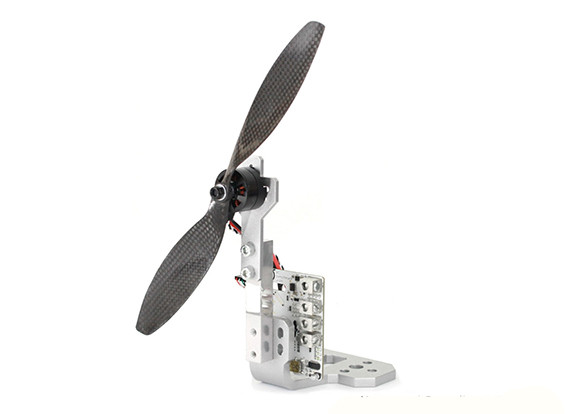
\includegraphics[width=0.5\textwidth]{Images/Propposed Aproach/TestBench.jpeg}
    \caption{Test bench used to measure the thrust and torque of the propeller.}
    \label{fig:Proposed Approach:Simulator:Testbench}
\end{figure}

With the test bench, we were able to measure the thrust and torque. Since, in real-world scenarios, propellers are either counterclockwise (CCW) or clockwise (CW), the data needed processing to make the curves symmetrical. This ensures that, in the simulation environment, no performance is lost by using the propeller in the wrong direction. The processed data is shown in Figure \ref{fig:Proposed Approach: Simulation: Motor Data}. 

The data exhibits a third-order curve, which was confirmed by analyzing the Mean Squared Error (MSE) between the real data and the fitted data. These MSE plots are shown in Figure \ref{fig:Proposed Approach: Simulation: Fitting Errors}. The analysis reveals that the third-order polynomial is the least complex model that accurately represents the data, as it significantly reduces the error compared to simpler models, while further increases in model complexity do not yield noticeable improvements.

\begin{figure}[H]
    \begin{subfigure}{0.5\textwidth}
        \centering
        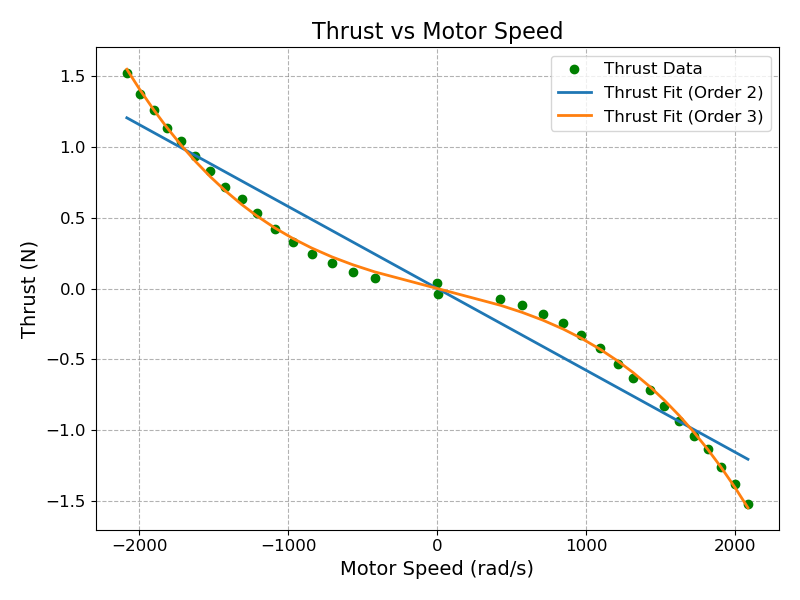
\includegraphics[width=0.9\textwidth]{Images/Propposed Aproach/thrust_vs_motor_speed.png}
        \caption{Thrust vs. motor speed.}
        \label{fig:proposed_approach_simulation_motor_data_thrust}
    \end{subfigure}
    \hfill
    \begin{subfigure}{0.5\textwidth}
        \centering
        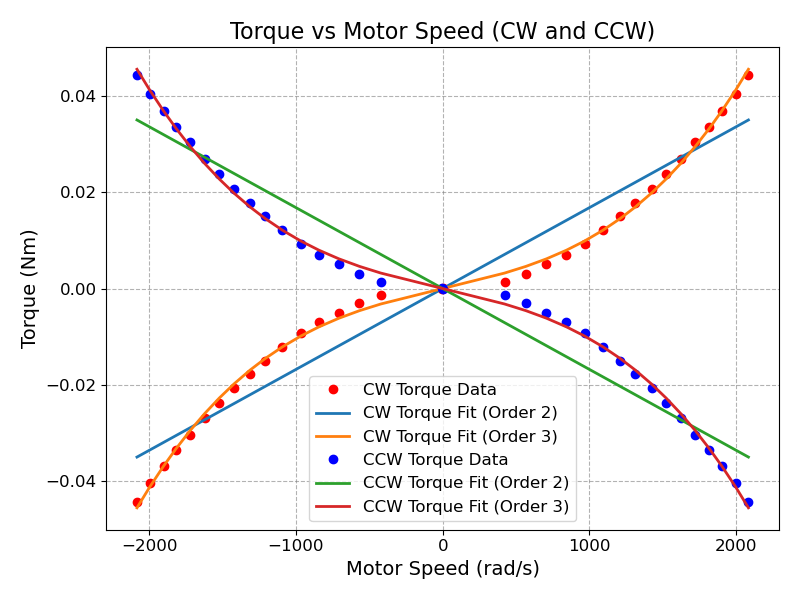
\includegraphics[width=0.9\textwidth]{Images/Propposed Aproach/torque_vs_motor_speed_CW_CCW.png}
        \caption{Torque vs. motor speed (CW and CCW).}
        \label{fig:proposed_approach_simulation_motor_data_torque}
    \end{subfigure}
    \caption{Thrust and Torque data.}
    \label{fig:Proposed Approach: Simulation: Motor Data}
\end{figure}

\begin{figure}[H]
    \begin{subfigure}{0.5\textwidth} 
        \centering
        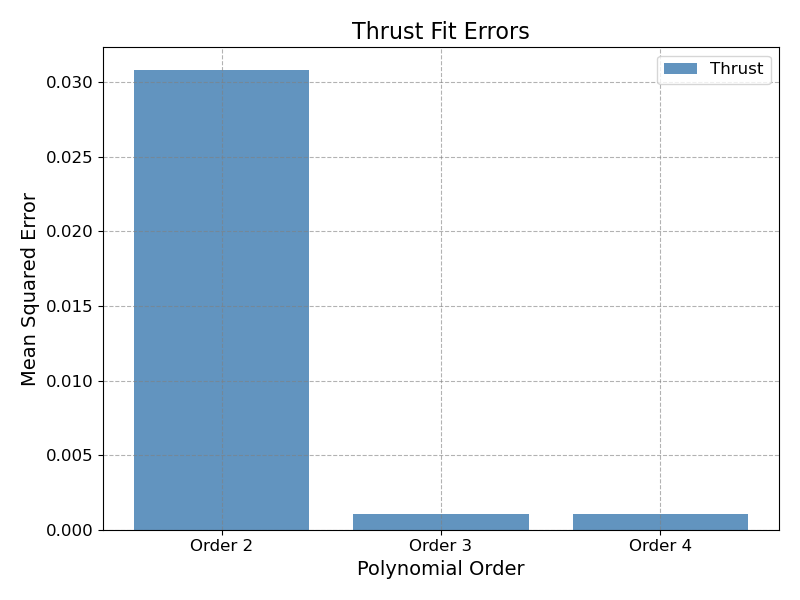
\includegraphics[width=0.9\textwidth]{Images/Propposed Aproach/thrust_errors.png}
        \caption{Thrust MSE between real data and fitted data.}
        \label{fig:Proposed Approach: Simulation: Thrust Errors}
    \end{subfigure} 
    \hfill
    \begin{subfigure}{0.5\textwidth}
        \centering
        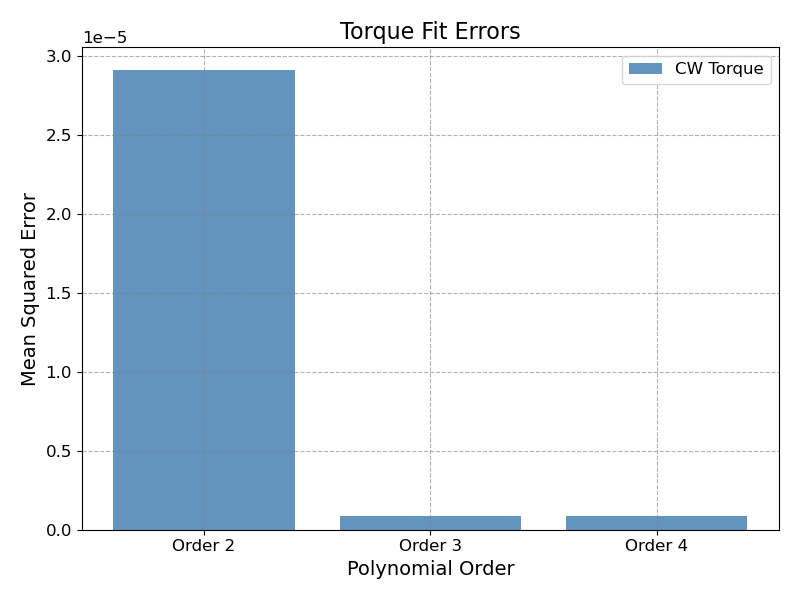
\includegraphics[width=0.9\textwidth]{Images/Propposed Aproach/torque_errors.png}
        \caption{Torque MSE between real data and fitted data.}
        \label{fig:Proposed Approach: Simulation: Torque Errors}
    \end{subfigure}
    \caption{MSE between the real data and the fitted curves.}
    \label{fig:Proposed Approach: Simulation: Fitting Errors}
\end{figure}
